\documentclass{article}\usepackage[]{graphicx}\usepackage[]{color}
% maxwidth is the original width if it is less than linewidth
% otherwise use linewidth (to make sure the graphics do not exceed the margin)
\makeatletter
\def\maxwidth{ %
  \ifdim\Gin@nat@width>\linewidth
    \linewidth
  \else
    \Gin@nat@width
  \fi
}
\makeatother

\definecolor{fgcolor}{rgb}{0.345, 0.345, 0.345}
\newcommand{\hlnum}[1]{\textcolor[rgb]{0.686,0.059,0.569}{#1}}%
\newcommand{\hlstr}[1]{\textcolor[rgb]{0.192,0.494,0.8}{#1}}%
\newcommand{\hlcom}[1]{\textcolor[rgb]{0.678,0.584,0.686}{\textit{#1}}}%
\newcommand{\hlopt}[1]{\textcolor[rgb]{0,0,0}{#1}}%
\newcommand{\hlstd}[1]{\textcolor[rgb]{0.345,0.345,0.345}{#1}}%
\newcommand{\hlkwa}[1]{\textcolor[rgb]{0.161,0.373,0.58}{\textbf{#1}}}%
\newcommand{\hlkwb}[1]{\textcolor[rgb]{0.69,0.353,0.396}{#1}}%
\newcommand{\hlkwc}[1]{\textcolor[rgb]{0.333,0.667,0.333}{#1}}%
\newcommand{\hlkwd}[1]{\textcolor[rgb]{0.737,0.353,0.396}{\textbf{#1}}}%
\let\hlipl\hlkwb

\usepackage{framed}
\makeatletter
\newenvironment{kframe}{%
 \def\at@end@of@kframe{}%
 \ifinner\ifhmode%
  \def\at@end@of@kframe{\end{minipage}}%
  \begin{minipage}{\columnwidth}%
 \fi\fi%
 \def\FrameCommand##1{\hskip\@totalleftmargin \hskip-\fboxsep
 \colorbox{shadecolor}{##1}\hskip-\fboxsep
     % There is no \\@totalrightmargin, so:
     \hskip-\linewidth \hskip-\@totalleftmargin \hskip\columnwidth}%
 \MakeFramed {\advance\hsize-\width
   \@totalleftmargin\z@ \linewidth\hsize
   \@setminipage}}%
 {\par\unskip\endMakeFramed%
 \at@end@of@kframe}
\makeatother

\definecolor{shadecolor}{rgb}{.97, .97, .97}
\definecolor{messagecolor}{rgb}{0, 0, 0}
\definecolor{warningcolor}{rgb}{1, 0, 1}
\definecolor{errorcolor}{rgb}{1, 0, 0}
\newenvironment{knitrout}{}{} % an empty environment to be redefined in TeX

\usepackage{alltt}
%Required: You must have these
\usepackage{graphicx}
\usepackage{tabularx}
\usepackage{natbib}
\usepackage{pdflscape}
\usepackage{array}
\usepackage{authblk}
\usepackage{gensymb}
\usepackage{amsmath}
%\usepackage[backend=bibtex]{biblatex}
\usepackage[small]{caption}
\usepackage[section]{placeins}
\setkeys{Gin}{width=0.8\textwidth}
\setlength{\captionmargin}{30pt}
\setlength{\abovecaptionskip}{10pt}
\setlength{\belowcaptionskip}{10pt}

 \topmargin -1.5cm 
 \oddsidemargin -0.04cm 
 \evensidemargin -0.04cm 
 \textwidth 16.59cm
 \textheight 21.94cm 
 \parskip 7.2pt 
\renewcommand{\baselinestretch}{1.8} 	
\parindent 0pt
\usepackage{setspace}
\usepackage{lineno}

\renewcommand{\thetable}{S\arabic{table}}
\renewcommand{\thefigure}{S\arabic{figure}}

\bibliographystyle{..//..//sub_projs/refs/styles/besjournals.bst}
\usepackage{xr-hyper}
%\usepackage{hyperref}
\externaldocument{FLS_flobud}
\externaldocument{JOErev_resp_parII}
\title{Supporting Information: Differences between flower and leaf phenological responses to environmental variation drive shifts in spring phenological sequences of temperate woody plants}
\date{}
\author{}
\IfFileExists{upquote.sty}{\usepackage{upquote}}{}
\begin{document}
\maketitle
\linenumbers
\section*{Tables}

\begin{table}[!ht]

\begin{tabular}{llllll}
  \hline
  Species & Family  & flower-leaf sequence & pollination & bud type & habit  \\ 
  \hline
  \textit{Acer pensylvanicum}& Sapindaceae & flowers with/after leaves & wind/insect & mixed & understory tree\\
  \textit{Acer rubrum}& Sapindaceae & flowers before leaves & wind/insect & separate & canopy tree \\ 
   \textit{Acer saccharum}& Sapindaceae & flowers before/with leaves & wind/insect & mixed & canopy tree\\
    \textit{Betula alleghaniensis}& Betulaceae & flowers before leaves & wind & separate & canopy tree\\
  \textit{Corylus cornuta}& Betulaceae & flowers before leaves & wind & separate & shrub\\
  \textit{Comptonia peregrina}& Myrtaceae & flowers before leaves & wind & separate & shrub\\
  \textit{Ilex mucronata} & Aquifoliaceae & flowers with leaves & insect & mixed & shrub \\
   \textit{Ilex verticillata} & Aquifoliaceae & flowers after leaves & insect & mixed & shrub \\
   \textit{Prunus pensylvanica} & Rosaceae & flowers with leaves & insect & mixed & understory tree\\
   \textit{Prunus virginiana} & Rosaceae & flowers with/after leaves & insect & mixed & shrub \\
   \textit{Vaccinium corymbosum} & Ericaceae & flowers after leaves & insect & separate & shrub\\
   \textit{Viburnum acerifolium} & Adoxaceae & flowers after leaves & insect & mixed & shrub\\
   \hline
\end{tabular}
\caption{Descriptive flower-leaf sequences classifications and functional traits for 12 temperate woody species collected from Harvard Forest (Petersham, MA, USA) and included in the lab experiment.}
\label{tab:splist}
\end{table}

\begin{table}[ht]
\centering
\begin{tabular}{rlrrrr}
  \hline
 &  & Harvard Forest & sd & Chamber: 30 days & Chamber: 60 days \\ 
  \hline
1 & Utah Model & 979.64 & 248.34 & 720.00 & 1440.00 \\ 
  2 & Chill Hours & 1170.71 & 273.07 & 720.00 & 1440.00 \\ 
  3 & Dynamic Model & 86.56 & 16.64 & 21.25 & 43.50 \\ 
   \hline
\end{tabular}
\caption{Comparisons between the average amount of chilling accumulated by woody plants at Harvard Forest (Petersham, MA, USA) between 15 October and 15 April in the field (Harvard Forest) and our experimental treatments (Chamber: 30 days, Chamber: 60 days)  using three alternative methods for calculating chilling (Utah Model, Chill hours, Dynamic Model, \citep[see][]{Luedeling:2011ab} for details).}
 \label{tab:chillcomps}
 \end{table}

\begin{table}[ht]
\centering
\begin{tabular}{rrrrrrr}
  \hline
 & Estimate & Est.Error & Q2.5 & Q25 & Q75 & Q97.5 \\ 
  \hline
Intercept & 70.81 & 9.18 & 52.99 & 64.94 & 76.88 & 88.08 \\ 
  Chill & -30.41 & 5.40 & -40.45 & -33.89 & -27.15 & -19.25 \\ 
  Light & 5.87 & 5.13 & -4.17 & 2.42 & 9.16 & 15.92 \\ 
  Force & -17.76 & 5.21 & -28.21 & -21.10 & -14.29 & -8.22 \\ 
  Chill:Light & -5.17 & 4.35 & -13.62 & -8.03 & -2.31 & 3.56 \\ 
  Chill:Force & 12.37 & 4.84 & 2.62 & 9.26 & 15.51 & 21.85 \\ 
  Light:Force & -12.62 & 4.10 & -20.50 & -15.37 & -9.87 & -4.79 \\ 
   \hline
\end{tabular}
\caption{Mean (`Estimate') and quantile (`Q') estimates of effects of forcing temperature, chilling duration, and photoperiod and all two-way interactions (change in day of phenological event/ change in environmental cue; 30 days chilling/6\degree C forcing/4 hours photoperiod) on leaf budburst of 10 woody plant species from Bayesian hierarchical models.}
\label{tab:modelests}
\end{table}

\begin{table}[ht]
\centering
\begin{tabular}{rrrrrrr}
  \hline
 & Estimate & Est.Error & Q2.5 & Q25 & Q75 & Q97.5 \\ 
  \hline
Intercept & 77.53 & 9.92 & 58.14 & 71.05 & 83.88 & 97.18 \\ 
  Chill & -21.23 & 7.42 & -35.35 & -26.14 & -16.32 & -6.07 \\ 
  Light & -5.72 & 5.70 & -18.28 & -9.01 & -2.03 & 4.86 \\ 
  Force & -18.98 & 6.51 & -32.09 & -23.02 & -14.93 & -6.37 \\ 
  Chill:Light & -0.88 & 6.11 & -13.59 & -4.72 & 3.21 & 10.55 \\ 
  Chill:Force & 7.01 & 6.62 & -6.35 & 2.98 & 11.11 & 20.31 \\ 
  Light:Force & -5.61 & 6.42 & -19.08 & -9.51 & -1.46 & 6.37 \\ 
   \hline
\end{tabular}
\caption{Mean (`Estimate') and quantile (`Q') estimates of effects of forcing temperature, chilling duration, and photoperiod and all two-way interactions (change in day of phenological event/change in environmental cue; 30 days chilling/6\degree C forcing/4 hours photoperiod) on flowering of 10 woody plant species from Bayesian hierarchical models.}
\label{tab:modelests2}
\end{table}


\begin{table}[ht]
\centering
\begin{tabular}{rlrrrrrrll}
  \hline
 & Species & Estimate & error & Q2.5 & Q25 & Q75 & Q97.5 & phase & sequence \\ 
  \hline
1 & A. pensylvanicum & -10.71 & 3.92 & -17.87 & -13.48 & -8.19 & -2.28 & leaf budburst & first \\ 
  2 & A. pensylvanicum & -17.43 & 6.15 & -30.48 & -20.68 & -14.00 & -5.59 & flowering & second \\ 
  3 & A. rubrum & -16.76 & 7.25 & -33.11 & -20.21 & -13.09 & -2.88 & flowering & first \\ 
  4 & A. rubrum & -28.39 & 6.22 & -40.52 & -32.69 & -24.08 & -16.20 & leaf budburst & second \\ 
  5 & C. peregrina & -13.28 & 3.33 & -19.62 & -15.50 & -11.17 & -6.60 & flowering & first \\ 
  6 & C. peregrina & -15.47 & 3.69 & -23.06 & -17.82 & -13.01 & -8.53 & leaf budburst & second \\ 
  7 & C. cornuta & -15.55 & 4.50 & -24.71 & -18.13 & -12.87 & -6.79 & flowering & first \\ 
  8 & C. cornuta & -19.82 & 4.04 & -28.13 & -22.41 & -17.10 & -11.99 & leaf budburst & second \\ 
  9 & I. mucronata & -10.44 & 3.81 & -17.42 & -13.09 & -8.05 & -2.45 & leaf budburst & first \\ 
  10 & I. mucronata & -16.05 & 4.06 & -24.19 & -18.58 & -13.47 & -7.94 & flowering & second \\ 
  11 & I. verticillata & -8.66 & 3.73 & -15.58 & -11.19 & -6.19 & -1.12 & leaf budburst & first \\ 
  12 & I. verticillata & -20.43 & 10.72 & -43.88 & -25.92 & -14.18 & -2.14 & flowering & second \\ 
  13 & P. pensylvanica & -10.24 & 4.14 & -18.67 & -12.99 & -7.50 & -2.14 & leaf budburst & first \\ 
  14 & P. pensylvanica & -13.85 & 4.02 & -21.59 & -16.46 & -11.40 & -5.39 & flowering & second \\ 
  15 & P. virginiana & -26.68 & 5.11 & -37.14 & -30.02 & -23.09 & -17.20 & leaf budburst & first \\ 
  16 & P. virginiana & -23.69 & 7.67 & -40.07 & -28.74 & -17.84 & -10.95 & flowering & second \\ 
  17 & V. corymbosum & -7.06 & 3.85 & -14.45 & -9.62 & -4.56 & 0.66 & leaf budburst & first \\ 
  18 & V. corymbosum & -13.10 & 3.60 & -20.30 & -15.49 & -10.79 & -5.99 & flowering & second \\ 
  19 & V. acerifolium & -12.68 & 3.78 & -19.97 & -15.14 & -10.29 & -5.10 & leaf budburst & first \\ 
  20 & V. acerifolium & -21.60 & 8.52 & -39.63 & -26.63 & -16.00 & -6.85 & flowering & second \\ 
   \hline
\end{tabular}
\caption{Mean (`Estimate') and quantile (`Q') estimates of effects of forcing temperature and all two-way interactions (change in day of phenological event/ $\Delta$6\degree C) on budburst and flowering of 10 woody plant species from Bayesian hierarchical models under long photoperiod and long chilling duration experimental treatments.}
\label{tab:phh}

\end{table}




\section*{Figures}

 \begin{figure}[!ht]
    \centering
 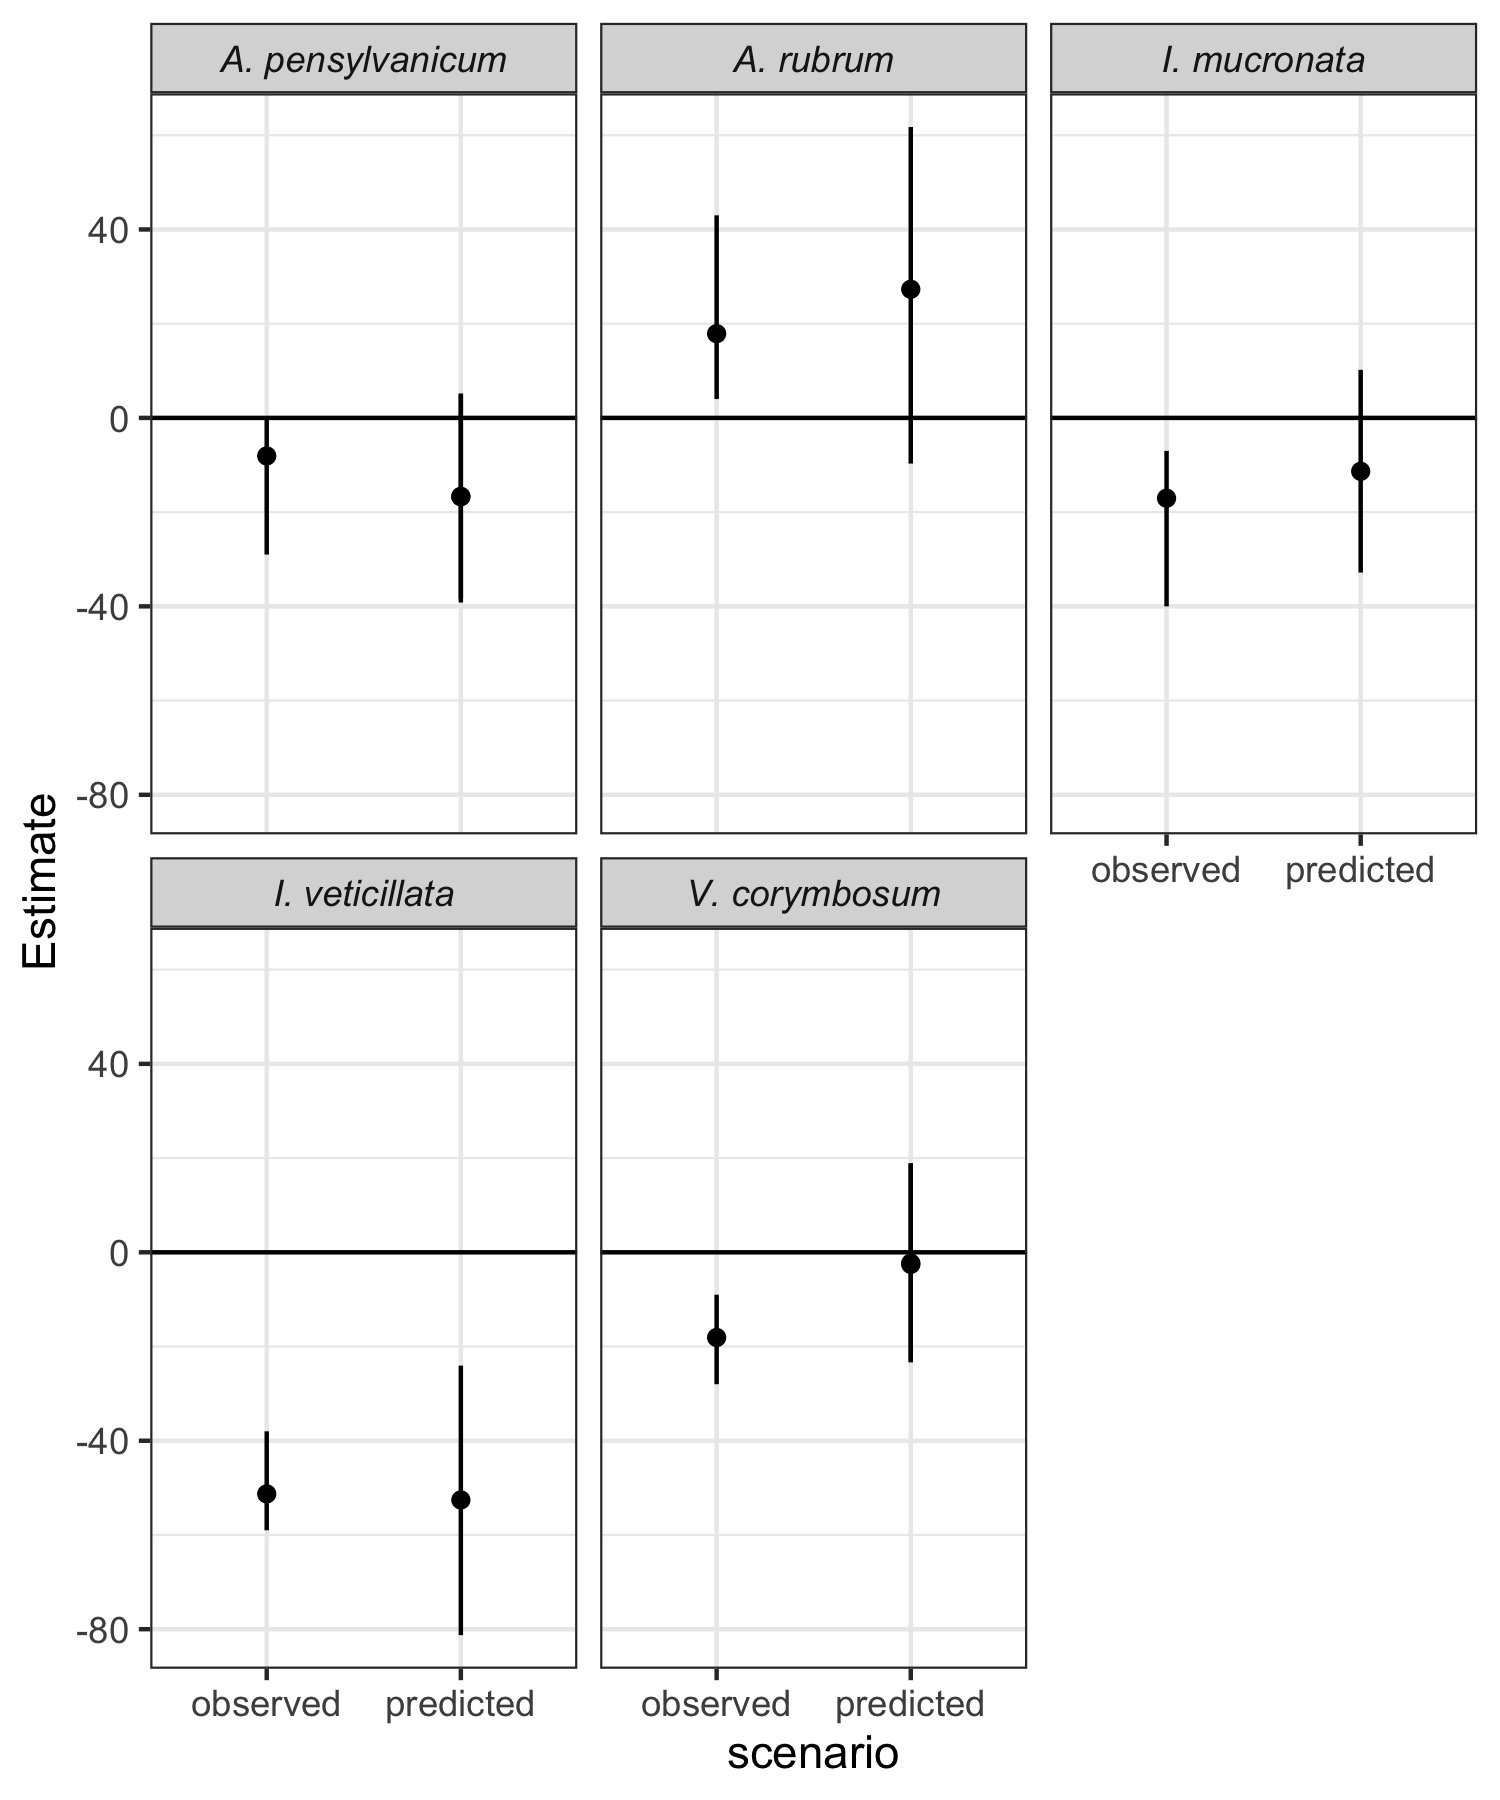
\includegraphics[width=.8\textwidth]{..//Plots/fieldmodcomparisions.jpeg}
    \caption{A comparison of the estimated mean flower-leaf sequence interphases (days between phenophase) for six woody plant species under artificial conditions designed to approximate ``average" field conditions and observed mean FLS interphases in the field at Harvard Forest in Pertersham MA. Dots represent means FLS interphase in both datasets, and lines represent the 50\% credible intervals and the full range of observations for our model predictions and Harvard Forest data respectively. Harvard Forest phenological records are from \citet{Okeefe2015}.}
    \label{fig:validate}
\end{figure}

 \begin{figure}[!ht]
    \centering
 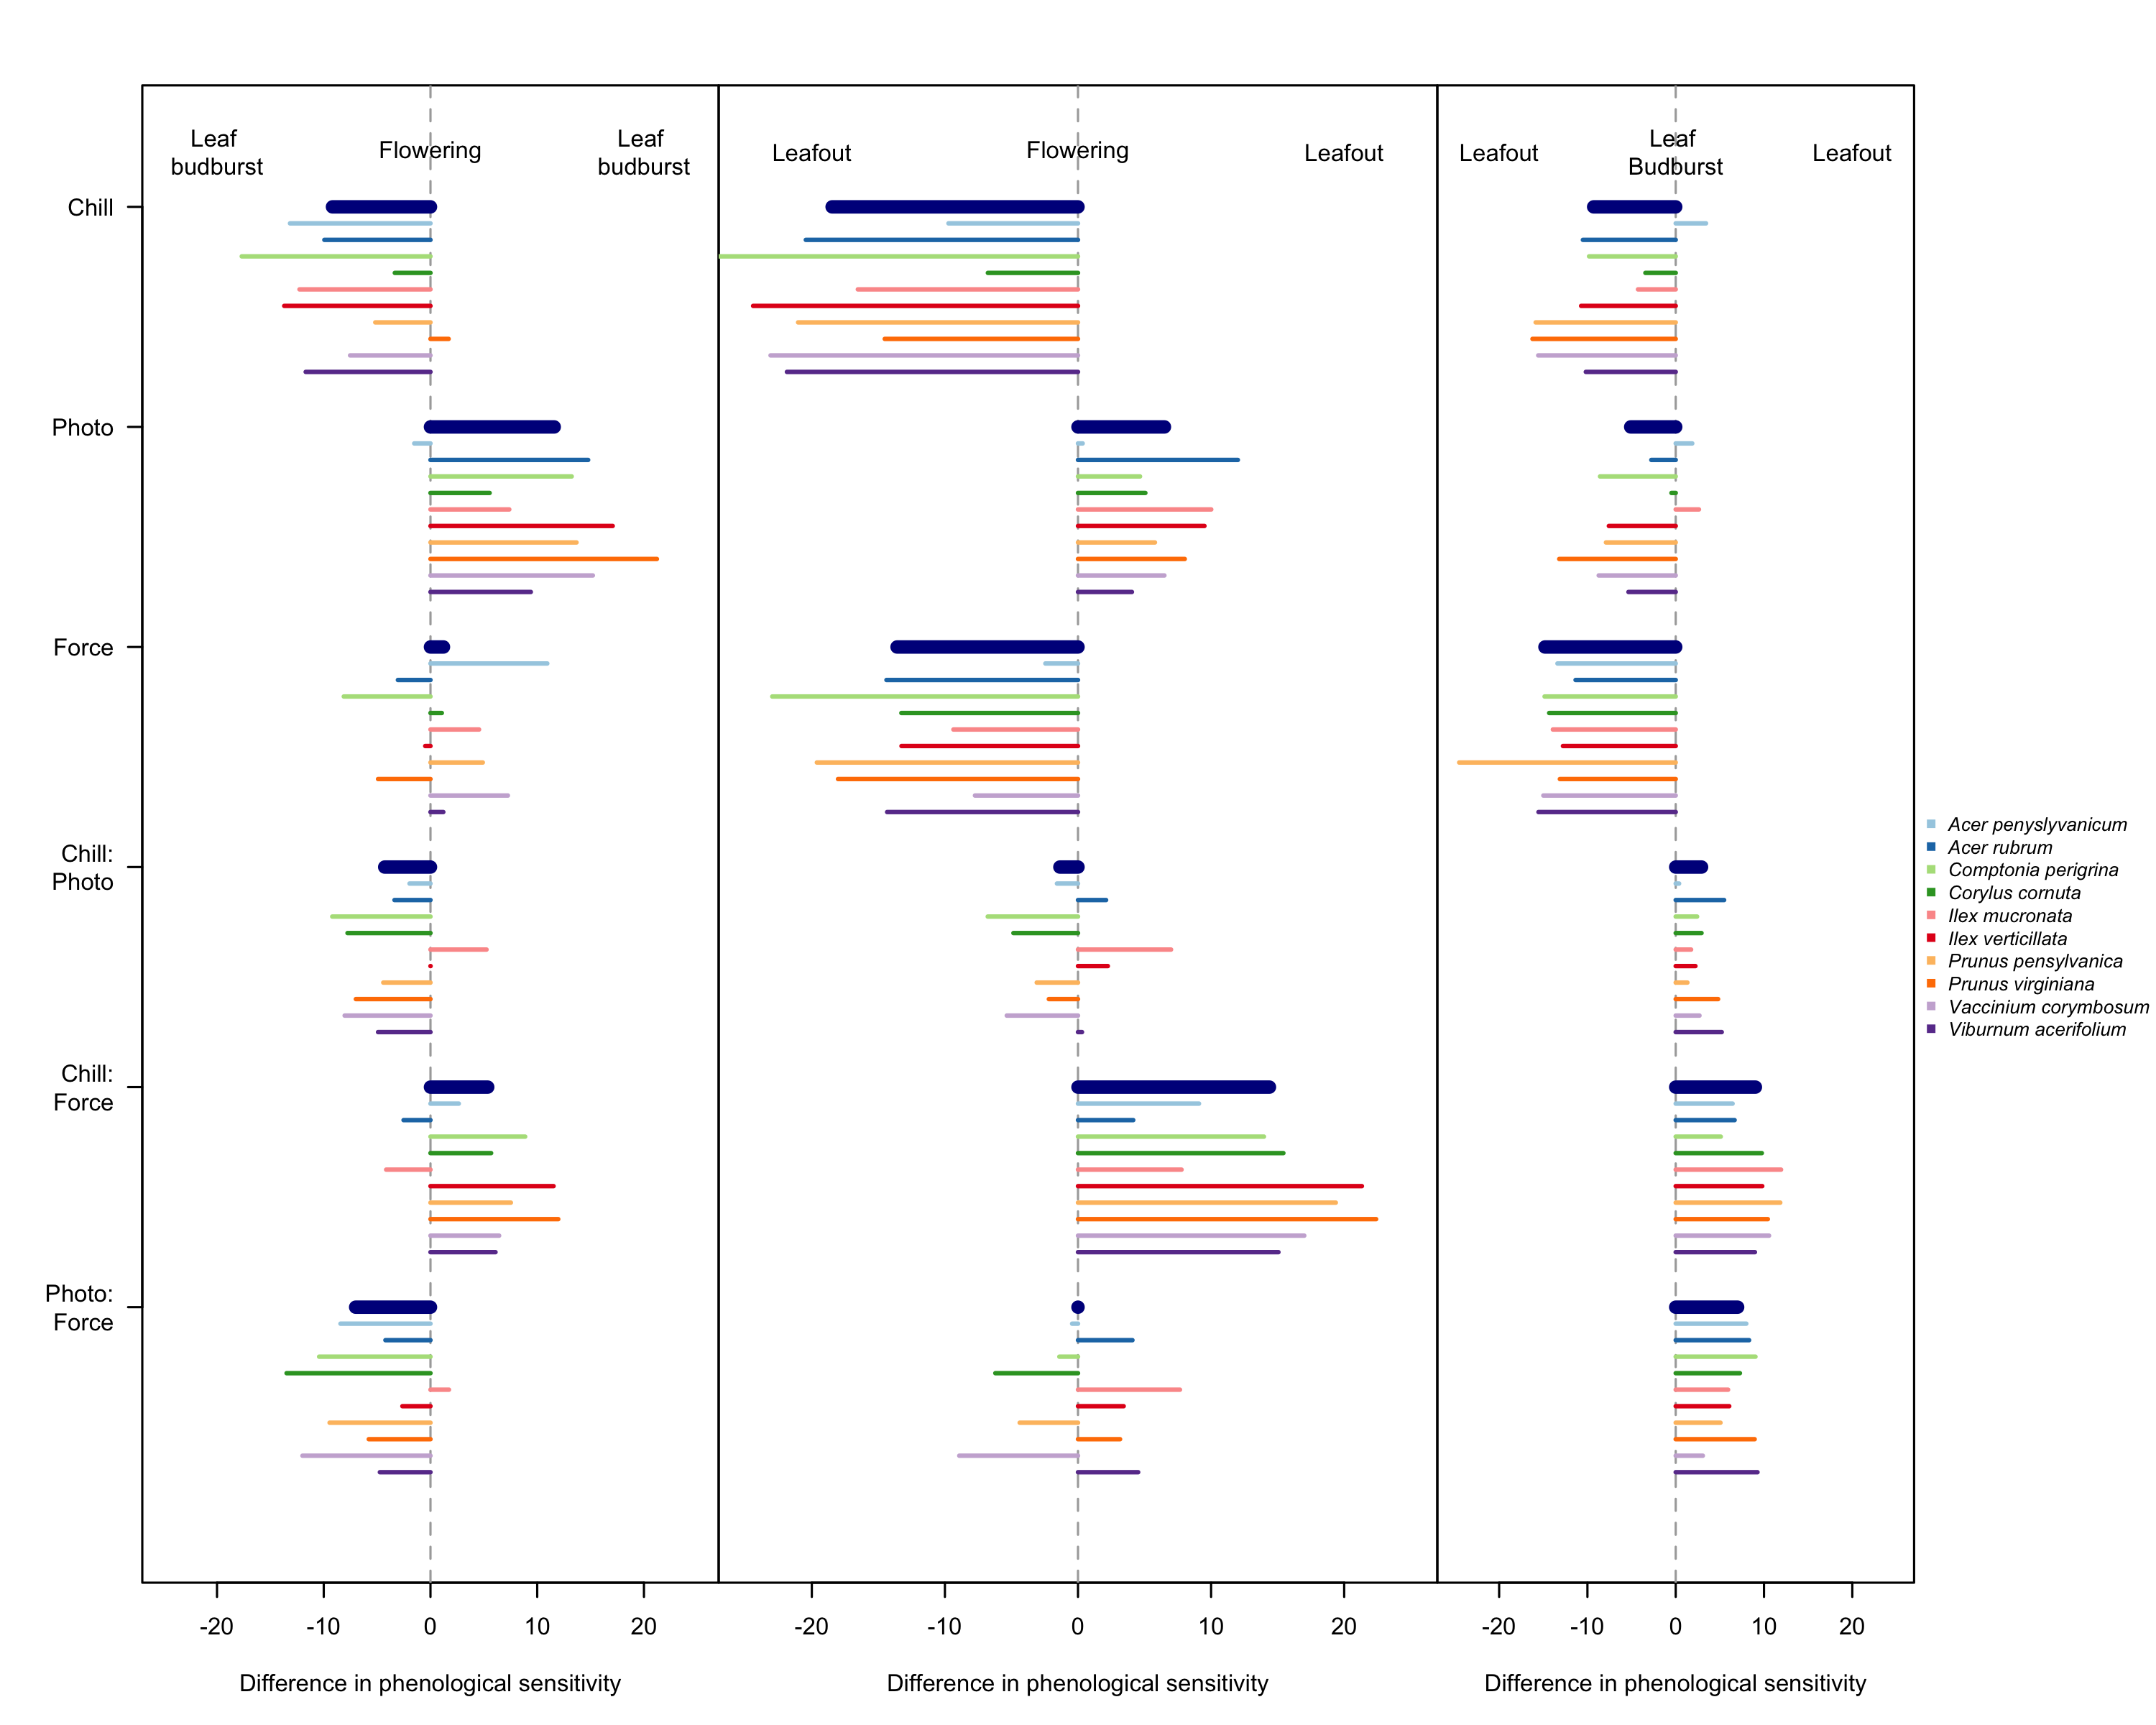
\includegraphics[width=\textwidth]{..//Plots/grover.png}
    \caption{The difference in mean effects of forcing temperature, chilling duration, and photoperiod between leaf budburst, leafout and flowering phenology of 10 temperate woody plant species collected from Harvard Forest (Petersham, MA, USA). Stronger advances in phenology are shown as negative numbers, and delays in phenology as positive numbers. The thicker blue bars depict the main effects for all species and thinner bars indicate the species-specific differences in the responses among phases.}
    \label{fig:altview}
\end{figure}



 \begin{figure}[!ht]
    \centering
 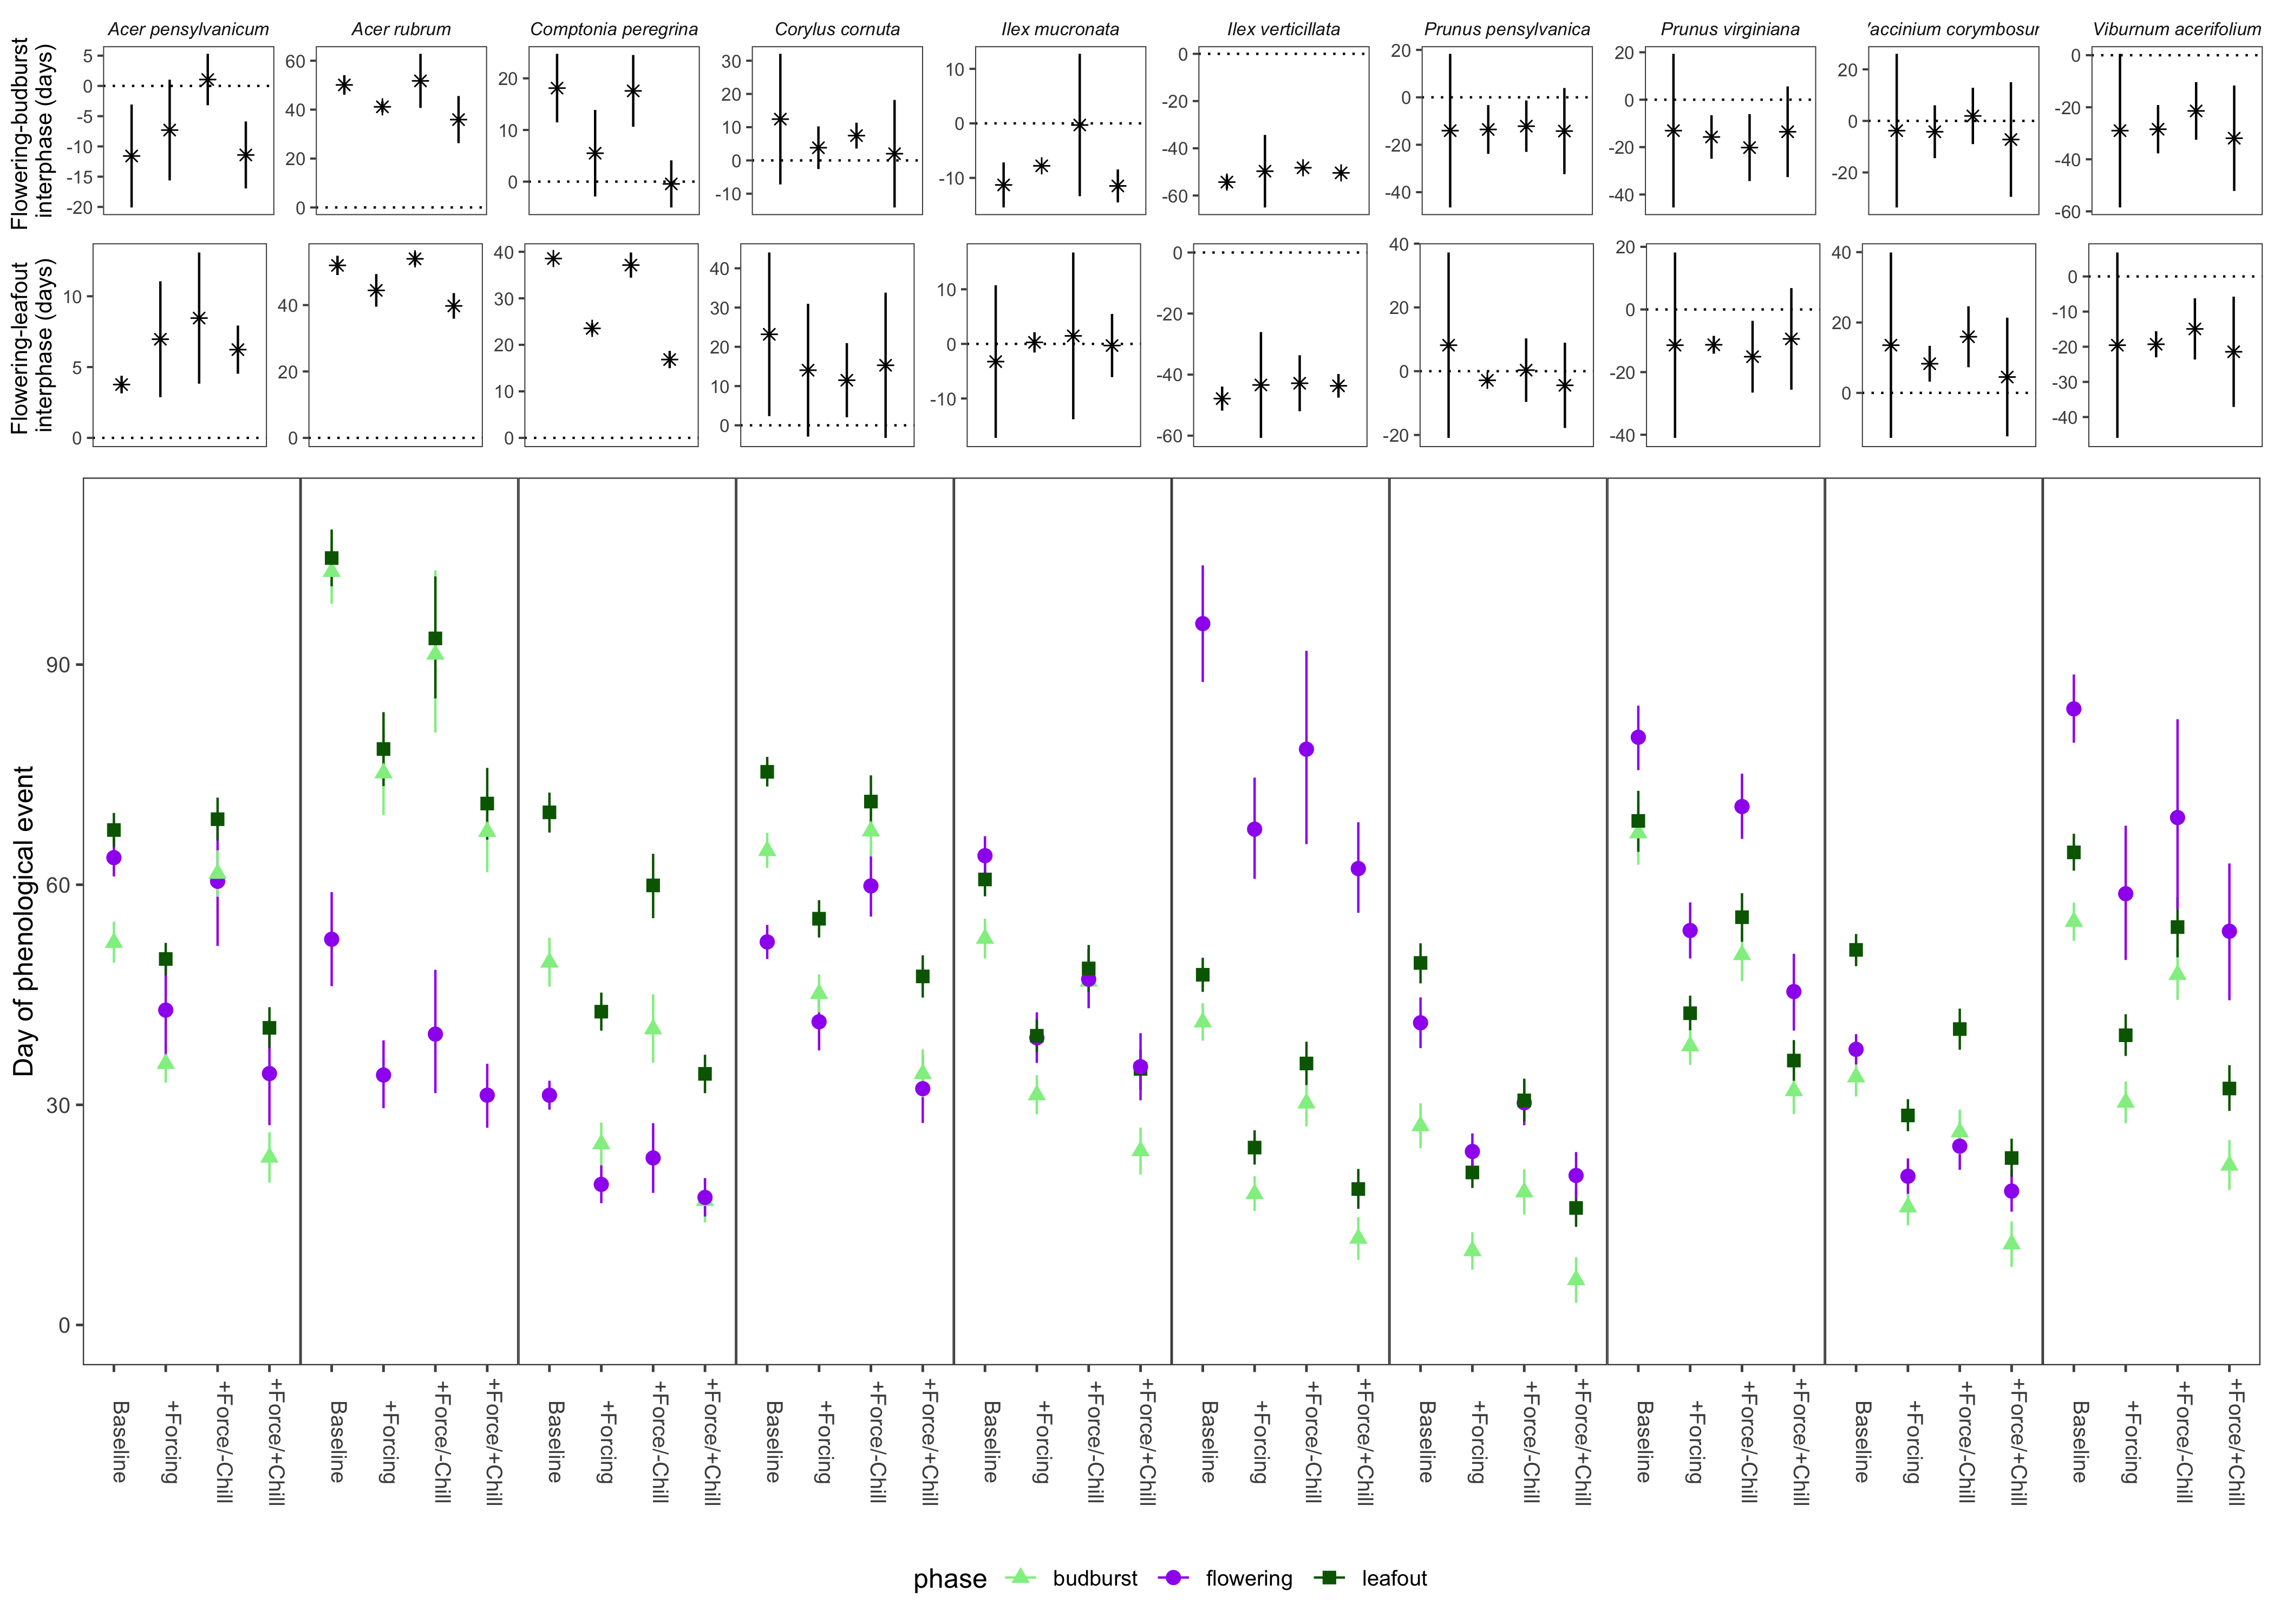
\includegraphics[width=\textwidth]{..//Plots/species_projections.png}
    \caption{Projected shifts in flower-leaf sequences under current environmental conditions (Baseline) and three climate change scenarios (increase forcing, increase forcing/decrease chilling, increase forcing/increase chilling) predict that FLS for 10 common temperate woody plant species. The top two rows show the mean time between flowering and vegetative phenological events (shapes) with 50\% credible intervals (lines). The bottom row shows the predicted event day for each phase. Predictions are based on posterior estimates from Bayesian hierarchical models comparing flowering (circles), leaf budburst (triangles) and leafout (squares) phenological responses to variable chilling duration and forcing temperatures. Shapes represent the mean estimates and lines represent the 50\% credible intervals. }
    \label{fig:preddy_sp}
\end{figure}


\section*{Supplemental Methods}
\subsection*{Simulations}
\noident To better understand the patterns of phenological sensitivity generated by the forcing hierarchy hypothesis (FHH) and the differential sensitivity hypothesis (DSH) respectively, we simulated the underlying physiology of each hypothesis, and used these simulations to generate flower and leaf phenology under two levels of chilling, forcing, and photoperiod in a fully factorial experimental design.\\

\noindent For the FHH we assigned flowering and leafing a critical heat sum threshold (F*) above which the phenological event would take place. We did this using a growing degree model with a base temperature of 5\degree C \citep{Fu:2014aa}. For the FHH simulations, we assigned flowering an F* of 200 GDDs and leafing an F* of 400 GDDs. In this scenario\linelabel{supple}, higher chilling and photoperiod reduced the F* value for each phenophase by 100 and 20 respectively.\\

\noindent For the DSH we assigned flowering and leafing identical F* values of 400. As in the previous scenario, we let increased chilling and photoperiod reduce the F* values, but these cues reduced the F* for leafing by 200 and 0 respectively and for flowering by 100 and 20.\\

\noindent We also included a third scenario that included both initial F* differences of the FHH (flowering: 200 and leafing: 400) and the differential response to chilling and photoperiod of the DSH (flowering: -100 chilling, -20 photoperiod, leafing -200 chilling, 0 photoperiod).

\bibliography{..//..//sub_projs/refs/hyst_outline.bib} 

\end{document}
